\documentclass[../main.tex]{subfiles}
\begin{document}
\chapter{Validazione del framework}
In questo capitolo verrà proposta una validazione di un deployment di test del framework Moon Cloud, mediante la valutazione della sicurezza tramite l'esecuzione del driver sviluppato a tutti i livelli dello stack cloud (infrastruttura, piattaforma, software). 

\section{Deployment di Moon Cloud}

Il deployment dell'ambiente di test è stato effettuato su un'architettura multi-layer così composta:
\begin{itemize}
    \item A livello di infrastruttura, un nodo fisico, Dell PowerEdge T430 equipaggiato con processore Intel(R) Xeon(R) CPU E5-2630 v4 (10 core fisici e 40 thread logici), 48GB di RAM e 5 dischi da 1TB ciascuno in configurazione RAID 1. Su questa macchina è stato installato il sistema operativo CentOS 7.2, e il software Open Stack Newton.
        Successivamente sono state create 3 macchine virtuali con sistema operativo CentOS 7.2, in un flavor con 4GB di RAM e 10GB di disco.
    \item A livello di piattaforma, un cluster Docker Swarm di 2 nodi per i componenti core di Moon Cloud. La terza macchina virtuale è stata utilizzata come nodo di esecuzione per un cluster di dimensione unaria.
    \item A livello software, i componenti di Moon Cloud: 7 servizi core, gestiti tramite container Docker sul cluster swarm e 3 microservizi per la gestione del nodo di esecuzione.\\
        \textbf{Componenti Core}
        \begin{itemize}
            \item API
            \item Database
            \item Repository
            \item Database \textit{time-series} per i risultati
            \item Evaluation Manager
            \item RabbitMQ per la comunicazione tra API e Container
            \item Traefik (reverse proxy) per l'esposizione delle API
        \end{itemize}
        \textbf{Componenti execution node e execution cluster}
        \begin{itemize}
            \item Execution Manager
            \item Monitor Execution Manager
            \item Traefik (reverse proxy) per l'esposizione di alcune tipologie di test
        \end{itemize}
\end{itemize}


\section{Sicurezza del deployment}
L'analisi della sicurezza è stata effettuata a livello di infrastruttura, analizzando le configurazioni sul sistema operativo del server fisico e le caratteristiche del setup OpenStack; a livello di piattaforma, analizzando le configurazioni del template utilizzato per le macchine virtuali Docker e i container Moon Cloud; a livello applicativo, analizzando la sicurezza nei meccanismi di integrazione dei vari componenti.
\subsection{Infrastruttura}
\subsubsection{Analisi OpenSCAP del server fisico}
\begin{comment}
test finished
started at 1496183480
ended at   1496184352
lasted -872 seconds
report available at
https://moonclouddashboard.blob.core.windows.net/pdfcontainer/f4a1943cff

\end{comment}
Il test è stato eseguito utilizzando il driver realizzato, specificando in input il documento XCCDF "\textit{ssg-centos7}" unitamente al profilo "\textit{nist-800-171-cui}".
Il documento \textit{JSON} dato in input al test è il seguente:
\begin{js}
{
    "read_ssh_configuration": {
    },
    "read_xccdf_configuration": {
        "xccdf":"ssg-centos7",
        "profile":"nist-800-171-cui",
        "fetch_remote_resources": true
    },
    "read_azure_configuration": {
    }
}
\end{js}

I risultati restituiti in output segnalano:
\begin{itemize}
    \item 119 valutazioni effettuate con successo
    \item 72 valutazioni fallite
\end{itemize}
\begin{figure}[H]
    \centering
    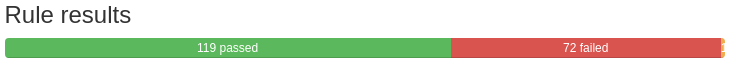
\includegraphics[width=10cm]{immagini/test_oscap_1.png}
\end{figure}

In particolare, delle 72 valutazioni fallite, 11 sono state catalogate da OpenSCAP con \textit{severit}y bassa, 50 con severity media e 11 con severity elevata; lo score della copertura XCCDF ottenuto è 71.17\%.
\begin{figure}[H]
    \centering
    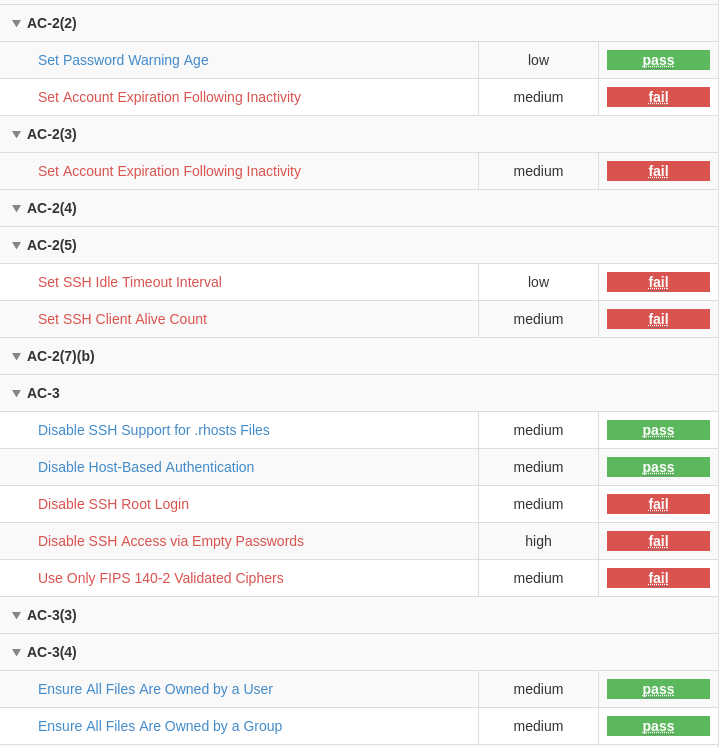
\includegraphics[width=10cm]{immagini/test_oscap_1_1.png}
    \caption{Estratto del report}\label{ref:report_oscap_1_1}
\end{figure}

In figura \ref{ref:report_oscap_1_1} è riportata una parte del report generato dal controllo sviluppato; il documento completo è disponibile in formato HTML all'indirizzo:\\
\textit{https://moonclouddashboard.blob.core.windows.net/pdfcontainer/f4a1943cff}
\\
o nel repository GIT\\
\textit{https://github.com/patriziotufarolo/tesi\_magistrale/}.

La valutazione delle \textit{OVAL} mediante il driver realizzato è durata 872 secondi; di seguito sono riportate le statistiche relative all'utilizzo delle risorse nell'esecuzione del test.
Queste sono state raccolte tramite il software \texttt{pidstat}, isolando esclusivamente i processi coinvolti nel processo di assessment.
\begin{figure}[H]
 \begin{minipage}[b]{6cm}
   \centering
   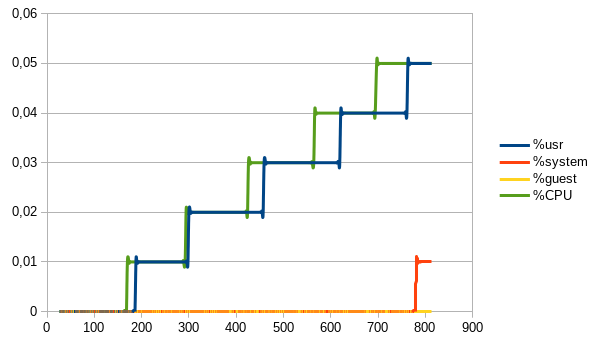
\includegraphics[width=6.6cm]{immagini/plot1cpu.png}
 \end{minipage}
 \hspace{2mm} \hspace{3mm}
 \begin{minipage}[b]{9cm}
  \centering
   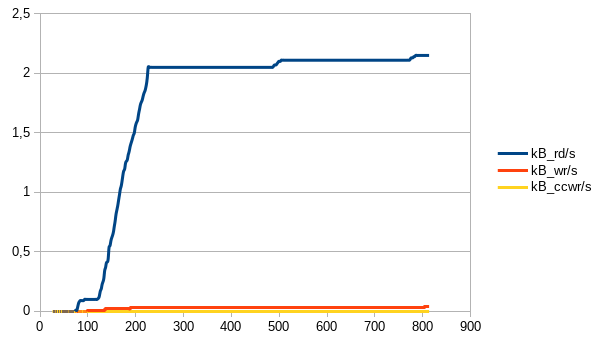
\includegraphics[width=6.6cm]{immagini/plot1io.png}
 \end{minipage}
 \caption{Utilizzo della CPU e carico IO}\label{ref:plot1cpuio}
\end{figure}
Dalla figura \ref{ref:plot1cpuio} è possibile notare come l'impatto del test sulle prestazioni del target sia minimo, registrando picchi di carico sulla CPU inferiori all'0.06\% per tutta la durata dell'esecuzione. Anche dal punto di vista delle operazioni di input/output il test si è dimostrato assolutamente non invasivo, registrando picchi in lettura di pochi KB. 
\begin{figure}[H]
 \begin{minipage}[b]{6cm}
   \centering
   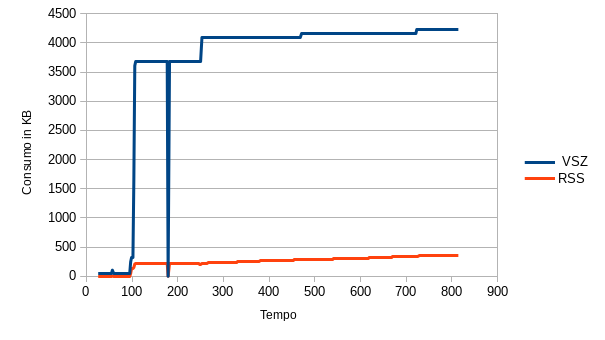
\includegraphics[width=6.6cm]{immagini/plot1mem.png}
 \end{minipage}
 \hspace{2mm} \hspace{3mm}
 \begin{minipage}[b]{9cm}
  \centering
   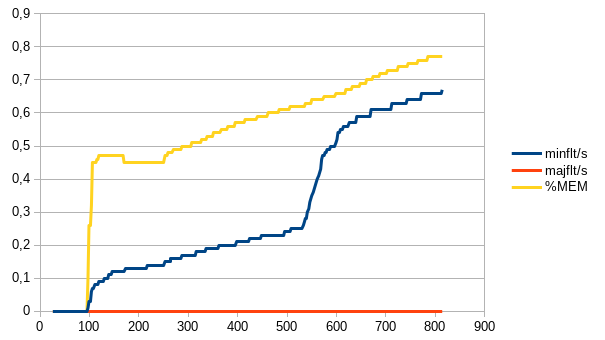
\includegraphics[width=6.6cm]{immagini/plot1mem2.png}
 \end{minipage}
 \caption{Utilizzo della memoria}\label{ref:plot1mem}
\end{figure}
In figura \ref{ref:plot1mem} è stato invece illustrato l'utilizzo della memoria durante l'esecuzione del test, che rimane sempre inferiore all'1\%. Anche in questo caso l'impatto prestazionale è minimo; il \textit{footprint} di \textit{OpenSCAP} e delle relative \textit{probes} non raggiunge i 5MB in memoria virtuale (\texit{VSZ}), rimanendo inoltre sotto i 500 KB in memoria RAM(\textit{RSS}).

Un test di questo tipo si presta particolarmente a scenari di esecuzione programmata e automatica, per effettuare monitoraggio continuativo.



\subsubsection{Analisi di OpenStack}
I documenti XCCDF forniti da OpenSCAP non sono risultati efficienti per l'assessment dei controlli di sicurezza per Open Stack, in quanto le definizioni \textit{OVAL} non sono state redatte
Questa sezione, pertanto, fa riferimento al paper "A Security Benchmark for OpenStack". Ogni raccomandazione citata nell'articolo è mappata sui requisiti FedRAMP corrispondenti. A causa del fatto che l'implementazione dei controlli automatici per alcuni di queste non sono disponibili, l'analisi è stata fatta in modo manuale ispezionando le configurazioni.
\begin{table}[h]
    \begin{tabulary}{\textwidth}{|c|c|c|}
    \hline
    Reccomendation & NIST Security Controls & \\ \hline

    [R1] Patch Levels. & SA-10(1) SI(3) & Passato \\ \hline
    [R2] Create and Enforce Account and Password Management Policies & AC-2 AC-2(3) AC-6 AC-7 AC-9 & Fallito \\ \hline
    [R3] Use a Central Directory for Authentication and Authorization. & AC-3 AC-17 & Fallito \\ \hline 
    [R4] Configure Firewalls to Restrict Access & CM-6 CM-7 & Passato \\ \hline
    [R5] Use TLS/SSL where Possible & Fallito \\ \hline
    [R6] Do Not Use Default Self-Signed Certificates. Non applicabile} \\ \hline
    [R7] Configure Centralized Remote Logging.} &
    Fallito} \\ \hline
    [R8] Maintain Time Synchronization Services.} &
    Passato} \\ \hline
    [R9] Review and Minimize Hypervisor Attack Surface.} &
    Non eseguito} \\ \hline
    [R10] Review and Minimize Virtual Machine Manager Attack Surface.} &
    Non eseguito} \\ \hline
    [R11] Use Templates to Deploy Virtual Machines.} &
Passato} \\ \hline
[R12] Disconnect unauthorized devices from Virtual Machines.} &
Non applicabile} \\ \hline
[R13] Disable MAC Address Changes and Promiscuous Mode on Guests.} Hypervisor or Network virtualizators should deny MAC address changes on the Vnic (\emph{Virtual})
Passato} \\ \hline
[R14] Ensure Network Isolation through VLANs.} 
Passato} \\ \hline
[R15] Port Groups Should not be Configured to Reserved VLANs.}
Passato} \\ \hline
[R16] Secure Access to Cloud Application Programming Interfaces.} 
Fallito} \\ \hline
[R17] Encrypt Data at Rest.} 
Fallito} \\ \hline
[R18] Establish Appropriate Resource Isolation.} 
Passato}
[R19] Evaluate Denial of Service Scenarios and Mitigations.} 
Fallito}
[R20] Do Not Use or Set Guest Customization Passwords.}
Passato}
[R21] Evaluate and Minimize Cloud Architecture Dependencie Non eseguito
[R22] Audit Sensible and Configuration Files. Fallito
[R23] Storage Reliability. Fallito
[R24] Data Remanence Avoidance Fallito}
\end{tabulary}
\end{table}

\subsection{Piattaforma}
\subsubsection{Analisi OpenSCAP sul template delle macchine virtuali}
test finished
started at 1496218136
ended at 1496218350
lasted -214 seconds

report available at
https://moonclouddashboard.blob.core.windows.net/pdfcontainer/b73210ae24
--

\subsubsection{Analisi del cluster Docker Swarm}

\subsection{Applicazione}
\subsubsection{Analisi dei componenti software}

L'analisi applicativa sulla piattaforma Moon Cloud è stata svolta analizzando le configurazioni dei servizi e la loro implementazione.


Di seguito i punti critici individuati:
\begin{itemize}
\end{itemize}




\end{document}
